\documentclass{article}

% ---------------------------------------------------------------------------
% STA5001 Bayesian & Computational Statistics - Final Project Report
% Official NeurIPS 2026 LaTeX template (course-mandated, single column).
% Student IDs and email addresses are placeholders in this working copy; see
% docs/final-delivery-status.md for the items that still need confirmation.
% ---------------------------------------------------------------------------

\usepackage[main, final]{neurips_2026}

\usepackage[utf8]{inputenc}
\usepackage[T1]{fontenc}
\usepackage{hyperref}
\usepackage{url}
\usepackage{booktabs}
\usepackage{amsfonts}
\usepackage{amsmath}
\usepackage{amssymb}
\usepackage{microtype}
\usepackage{xcolor}
\usepackage{graphicx}

\hypersetup{
  colorlinks=true,
  linkcolor=[rgb]{0.00,0.08,0.45},
  citecolor=[rgb]{0.00,0.08,0.45},
  urlcolor=[rgb]{0.00,0.08,0.45},
  pdfborder={0 0 0},
  breaklinks=true,
  bookmarksnumbered=true,
  pdftitle={Bayesian weather associations and daily time structure in multi-city bike share},
  pdfauthor={XUE Yantong, WANG Ziyu, and ZHAO Jiashen},
  pdfsubject={STA5001 Final Project},
}

\graphicspath{{../figures/}}

% 交付用文档输入，由人工依据已保存的正式结果整理。
% 整理日期 2026-10-01。运行标识 formal_20260930。
% 数值来源：runs/formal_20260930/<model>/<fold>/ 下的 effects.json、diagnostics.json、
% metrics_overall.json、residual_summary.json、prior_predictive.json；
% tables/paired_comparison.json；logs/review-20261001/ 下的独立核验记录。
% 宏名中的 MZero / MOne / MTwo 分别对应 M0 / M1 / M2，Sel 表示开发窗口选定的模型。

% ---------------------------------------------------------------- 选模与数据范围
\newcommand{\SelModel}{M2}
\newcommand{\PanelCityCount}{29}
\newcommand{\PanelRows}{10{,}578}
\newcommand{\CityCount}{25}
\newcommand{\PredCityCount}{23}
\newcommand{\PrimaryRows}{9{,}120}
\newcommand{\PredictionRows}{8{,}393}
\newcommand{\DevOneTrain}{4{,}529}
\newcommand{\DevTwoTrain}{5{,}817}
\newcommand{\FinalTrain}{7{,}105}
\newcommand{\TestRows}{1{,}288}
\newcommand{\BlockDays}{56}
\newcommand{\SelDevMeanWis}{0.1421}
\newcommand{\MOneDevMeanWis}{0.1606}
\newcommand{\MZeroDevMeanWis}{0.1692}
\newcommand{\SelGapToMOne}{13.1}
\newcommand{\SelGapToMZero}{19.1}

% ---------------------------------------------------------------- 采样与收敛
\newcommand{\CoreFits}{11}
\newcommand{\CoreMaxRhat}{1.00894}
\newcommand{\CoreMinEss}{426.7}
\newcommand{\CoreMinTailEss}{668.9}
\newcommand{\WarmupDraws}{3{,}000}

% ---------------------------------------------------------------- 时间相关诊断（开发折 1）
\newcommand{\MZeroDevOneLagOne}{0.317}
\newcommand{\MOneDevOneLagOne}{0.329}
\newcommand{\MTwoDevOneLagOne}{0.066}
\newcommand{\MTwoDevTwoLagOne}{-0.003}
\newcommand{\MTwoFinalLagOne}{-0.036}
\newcommand{\MZeroDevOneTrainCov}{90.1}
\newcommand{\MTwoDevOneTrainCov}{90.8}

% ---------------------------------------------------------------- 全期关联：M0（25 城市）
\newcommand{\RainMZeroMed}{-19.98}
\newcommand{\RainMZeroLo}{-21.07}
\newcommand{\RainMZeroHi}{-18.89}
\newcommand{\RainSupportMZeroMed}{-16.40}
\newcommand{\RainSupportMZeroLo}{-17.28}
\newcommand{\RainSupportMZeroHi}{-15.53}
\newcommand{\TempMZeroMed}{5.22}
\newcommand{\TempMZeroLo}{3.67}
\newcommand{\TempMZeroHi}{6.76}
\newcommand{\TempSupportMZeroMed}{19.89}
\newcommand{\TempSupportMZeroLo}{17.44}
\newcommand{\TempSupportMZeroHi}{22.47}
\newcommand{\PeakCitiesMZero}{15}
\newcommand{\ExtrapCitiesMZero}{1}
\newcommand{\RainMZeroMinPNeg}{0.998}
\newcommand{\RainMZeroCityMin}{-33.84}
\newcommand{\RainMZeroCityMax}{-8.03}

% ---------------------------------------------------------------- 全期关联：M2（25 城市）
\newcommand{\RainMTwoMed}{-20.21}
\newcommand{\RainMTwoLo}{-21.37}
\newcommand{\RainMTwoHi}{-18.99}
\newcommand{\RainSupportMTwoMed}{-16.99}
\newcommand{\RainSupportMTwoLo}{-18.02}
\newcommand{\RainSupportMTwoHi}{-15.95}
\newcommand{\TempMTwoMed}{6.16}
\newcommand{\TempMTwoLo}{4.12}
\newcommand{\TempMTwoHi}{8.32}
\newcommand{\TempSupportMTwoMed}{14.04}
\newcommand{\TempSupportMTwoLo}{11.11}
\newcommand{\TempSupportMTwoHi}{17.27}
\newcommand{\PeakCitiesMTwo}{5}
\newcommand{\ExtrapCitiesMTwo}{1}
\newcommand{\RainMTwoMinPNeg}{0.984}
\newcommand{\RainMTwoCityMin}{-36.18}
\newcommand{\RainMTwoCityMax}{-10.05}
\newcommand{\PhiMTwoMed}{0.498}
\newcommand{\PhiMTwoLo}{0.147}
\newcommand{\PhiMTwoHi}{0.912}
\newcommand{\NuMTwoMed}{2.76}
\newcommand{\NuMTwoLo}{2.55}
\newcommand{\NuMTwoHi}{3.01}
\newcommand{\ObsUtciMinC}{-37.8}
\newcommand{\ObsUtciMaxC}{34.3}

% ---------------------------------------------------------------- 预测评分（56 天块预测，城市等权 WIS）
\newcommand{\MZeroDevOneWis}{0.1338}
\newcommand{\MZeroDevTwoWis}{0.2046}
\newcommand{\MZeroFinalWis}{0.1957}
\newcommand{\MOneDevOneWis}{0.1320}
\newcommand{\MOneDevTwoWis}{0.1893}
\newcommand{\MOneFinalWis}{0.3690}
\newcommand{\MTwoDevOneWis}{0.1265}
\newcommand{\MTwoDevTwoWis}{0.1577}
\newcommand{\MTwoFinalWis}{0.3394}
\newcommand{\MTwoDevOneStepWis}{0.1084}
\newcommand{\MTwoDevTwoStepWis}{0.1238}
\newcommand{\MTwoFinalStepWis}{0.2085}
\newcommand{\MZeroFinalStepWis}{0.1957}
\newcommand{\MZeroFinalStepCov}{75.7}
\newcommand{\MTwoFinalBlockCov}{60.5}
\newcommand{\MTwoFinalStepCov}{72.0}
\newcommand{\MZeroFinalBlockCov}{75.5}
\newcommand{\MTwoFinalBlockWidth}{1.095}
\newcommand{\MZeroFinalBlockWidth}{0.844}

% ---------------------------------------------------------------- 配对区间（M2 减 M0，7 日区块）
\newcommand{\PairDevOneLo}{-0.0153}
\newcommand{\PairDevOneHi}{0.0011}
\newcommand{\PairDevTwoLo}{-0.0675}
\newcommand{\PairDevTwoHi}{-0.0231}

% ---------------------------------------------------------------- 末段基线点预测（对数尺度 MAE）
\newcommand{\BaseConstFinalMae}{0.5551}
\newcommand{\BaseNaiveFinalMaeBlock}{0.4252}
\newcommand{\BaseNaiveFinalMaeStep}{0.3421}
\newcommand{\BaseOlsFinalMae}{0.5208}
\newcommand{\BaseArOlsFinalMaeBlock}{0.5192}
\newcommand{\BaseArOlsFinalMaeStep}{0.3197}
\newcommand{\MZeroFinalMaeBlock}{0.3207}
\newcommand{\MZeroFinalMaeStep}{0.3207}
\newcommand{\MTwoFinalMaeBlock}{0.5547}
\newcommand{\MTwoFinalMaeStep}{0.3601}

% ---------------------------------------------------------------- 开发折 1 基线点预测
\newcommand{\BaseConstDevOneMae}{0.3757}
\newcommand{\BaseNaiveDevOneMaeBlock}{0.2602}
\newcommand{\BaseNaiveDevOneMaeStep}{0.2298}
\newcommand{\BaseOlsDevOneMae}{0.3314}
\newcommand{\BaseArOlsDevOneMaeBlock}{0.3309}
\newcommand{\BaseArOlsDevOneMaeStep}{0.2553}
\newcommand{\MZeroDevOneMaeBlock}{0.2571}
\newcommand{\MTwoDevOneMaeBlock}{0.2503}
\newcommand{\MTwoDevOneMaeStep}{0.2104}

% ---------------------------------------------------------------- 先验与先验预测
\newcommand{\PriorNegIntercept}{1.15}
\newcommand{\PriorNegJoint}{3.50}
\newcommand{\PriorLogLow}{-5.90}
\newcommand{\PriorLogHigh}{19.46}
\newcommand{\ObsLogHigh}{11.65}
\newcommand{\TrainNegative}{0.056}

% ---------------------------------------------------------------- 天气先验尺度敏感性（M2，开发折 1）
\newcommand{\SensRainBase}{-18.18}
\newcommand{\SensRainHalf}{-18.17}
\newcommand{\SensRainDouble}{-18.15}
\newcommand{\SensTempBase}{7.49}
\newcommand{\SensTempHalf}{7.46}
\newcommand{\SensTempDouble}{7.49}

% ---------------------------------------------------------------- 预测积分稳定性（M2）
\newcommand{\IntegDevOneWis}{0.1265}
\newcommand{\IntegFinalWis}{0.3373}
\newcommand{\IntegDevOneWisNew}{0.12653}
\newcommand{\IntegDevOneWisSaved}{0.12649}
\newcommand{\IntegFinalWisNew}{0.33731}
\newcommand{\IntegFinalWisSaved}{0.33942}
\newcommand{\IntegFinalDensity}{-1.510}
\newcommand{\DensityStabilityDevOne}{0.126}
\newcommand{\DensityStabilityFinal}{0.363}

% ---------------------------------------------------------------- 开发折 1 的关联（用于说明规格依赖）
\newcommand{\RainMZeroDevOneMed}{-18.17}
\newcommand{\RainMOneDevOneMed}{-17.94}
\newcommand{\RainMTwoDevOneMed}{-18.18}
\newcommand{\TempMZeroDevOneMed}{11.35}
\newcommand{\TempMZeroDevOneLo}{9.72}
\newcommand{\TempMZeroDevOneHi}{12.99}
\newcommand{\TempMOneDevOneMed}{10.07}
\newcommand{\TempMOneDevOneLo}{8.25}
\newcommand{\TempMOneDevOneHi}{12.01}
\newcommand{\TempMTwoDevOneMed}{7.49}
\newcommand{\TempMTwoDevOneLo}{5.47}
\newcommand{\TempMTwoDevOneHi}{9.65}

% ---------------------------------------------------------------- 城市趋势（M2，末段折）
\newcommand{\TrendCityMedian}{0.17}
\newcommand{\TrendCityMin}{0.06}
\newcommand{\TrendCityMax}{0.39}
\newcommand{\TrendWindowLow}{1.55}
\newcommand{\TrendWindowHigh}{2.10}
\newcommand{\TrendLogLow}{0.26}
\newcommand{\TrendLogHigh}{0.36}


\title{Bayesian weather associations and daily time structure\\in multi-city dock-based bike share}

\author{%
  XUE Yantong \\
  Student ID: 00000000 \\
  Email: student1@example.com \\
  School of Data Science, CUHK-Shenzhen
  \And
  WANG Ziyu \\
  Student ID: 00000000 \\
  Email: student2@example.com \\
  School of Data Science, CUHK-Shenzhen
  \And
  ZHAO Jiashen \\
  Student ID: 00000000 \\
  Email: student3@example.com \\
  School of Data Science, CUHK-Shenzhen
}

\begin{document}

\maketitle

\begin{abstract}
Weather is one of the few drivers a bike-share operator cannot control. This project continues the
midterm panel: a public daily dataset derived from the release behind \citet{bean2021weather}, with
\PanelCityCount{} systems and \PanelRows{} city-days. We estimate hierarchical Student-$t$
regressions with city weather coefficients drawn from a common population. The association analysis
keeps \CityCount{} continuously operating systems and the prediction evaluation keeps
\PredCityCount{} covering all of 2017. Precipitation is the stable result: a $+10$ mm step from the
city median is associated with a \RainMTwoMed\% change in the conditional median of
$(1+\text{usage})$ under M2 (95\% interval $[\RainMTwoLo,\RainMTwoHi]$) and \RainMZeroMed\% under M0. The temperature association is positive over the full period under both
specifications, but the interior peak moves with the specification, so we name no optimal
temperature. M2 shows lower lag-one correlation in its innovation residuals and lower prediction
scores in the development windows, but its block forecast on the pre-specified final window is worse
than the archived model, with 90\% coverage of \MTwoFinalBlockCov\%. The specifications differ in
several structural components, so the contribution of AR(1) alone is not established.
\end{abstract}

% ===========================================================================
\section{Introduction}
% ===========================================================================

Bike-share operators plan rebalancing, pricing and maintenance around demand that moves with the
weather. The comparative study of \citet{bean2021weather} fits a separate generalised additive model
to each of forty cities and reports a thermal response that usually peaks near $27$--$28^\circ$C and
a negative rainfall response. Fitting each city separately is a natural first step, and it leaves
two questions open. First, with roughly one year of daily data per city, how much of the apparent
city-to-city spread in weather sensitivity is signal rather than noise? Second, does treating days
as exchangeable observations leave structure in the residuals that matters once the model is asked
to predict?

We address three questions, using the same dataset and the same scientific problem as the midterm
project.

\begin{enumerate}
  \item Once calendar effects and seasonal variation are controlled, what is the association
        between precipitation and daily usage, and how much does it differ between cities?
  \item What are the direction, shape and uncertainty of the temperature association, and how do
        they change across model specifications?
  \item What do calendar, trend and AR(1) (first-order autoregressive) residual structure change
        about diagnostics and prediction in the development windows, and does the final window
        support extending those results?
\end{enumerate}

The associations are observational. We do not identify causal effects, we do not estimate climate
adaptation, and because both prediction tasks condition on realised weather, we make no claim about
operational forecasting that includes weather-forecast error.

% ===========================================================================
\section{Data and evaluation design}
% ===========================================================================

\paragraph{Panel and rosters.}
The frozen input is a daily panel derived from the Mendeley Data release
\citep{mendeley2021bikeshare} (Version 1, CC BY 4.0) that accompanies \citet{bean2021weather}.
Hourly hires inferred from station inventory snapshots are aggregated to local dates and paired with
daily summaries of the Universal Thermal Climate Index (UTCI), a thermal-stress index that combines
air temperature, humidity, wind and radiation and is not the same quantity as air temperature,
together with daily precipitation from the Copernicus Climate Data Store \citep{cds2020utci}. The
panel holds \PanelRows{} city-days for \PanelCityCount{} systems with no duplicate city-date keys,
no missing cells and no negative values. Usage is inferred from inventory changes, may include
rebalancing moves, and is not a count of individual trips.

Three scopes are fixed by the frozen metadata rather than by any result, and
Figure~\ref{fig:overview} in the appendix shows them city by city. The association analysis keeps
the \CityCount{} systems with \texttt{continuous\_system} equal to one, that is, systems that record
hires on at least 99\% of their analysis days; these contribute \PrimaryRows{} city-days. The
prediction evaluation keeps the \PredCityCount{} of those systems whose study period spans
2017-01-02 to 2017-12-31, which excludes Kaohsiung and Melbourne because they cover 2016-07-02 to
2017-06-30; the roster contributes \PredictionRows{} city-days. The prediction roster is therefore
conditioned on full-period activity, and it is not re-selected using test-period usage.

\paragraph{Time splits.}
Every model is trained only on observations at or before a common cutoff, so a model predicting one
city's June cannot learn from another city's November. We use two development folds and one
pre-specified final fold, each with a \BlockDays-day test block: cutoff 2017-07-16 with test
2017-07-17 to 2017-09-10; cutoff 2017-09-10 with test 2017-09-11 to 2017-11-05; and cutoff
2017-11-05 with test 2017-11-06 to 2017-12-31. Training rows are \DevOneTrain, \DevTwoTrain{} and
\FinalTrain; every test block is $\PredCityCount\times\BlockDays=\TestRows$ rows. The final block was
included in the full-period midterm exploratory analysis, so its observations were already available
before the final project. We report this pre-specified evaluation with that disclosure. All centring
constants, scales and moderators are computed from training rows only.

\paragraph{Prediction tasks.}
The \emph{block} task fixes a start date and predicts the next \BlockDays{} days without reading any
realised usage after the start, propagating the residual state forward from the posterior. The
\emph{one-step} task predicts day $t$ from realised usage through day $t-1$, with the parameters
fixed at the start of the window. Both use realised weather, so neither includes weather-forecast
error, and the two tasks are not directly comparable because they condition on different information.

\paragraph{Metrics.}
We report the weighted interval score (WIS), the log-scale mean absolute error (MAE) and the 90\%
interval coverage, all on the $\log(1+\text{usage})$ scale and aggregated with equal city weights, so
that no single large system dominates. The appendix gives the full definitions, the additional
normalised error, and the four baselines. Because the multi-step intervals of the seasonal naive and
AR-OLS baselines do not accumulate future innovation uncertainty, we use the baselines only for
point-forecast comparison and do not base any model-superiority claim on their interval scores,
densities or coverages.

% ===========================================================================
\section{Models and priors}
% ===========================================================================

All models share the response $y_{it}=\log(1+U_{it})$ for city $i$ on local date $t$, a Student-$t$
likelihood with a shared degrees-of-freedom parameter $\nu$ and a city-specific scale $\sigma_i$, and
the linear predictor
\begin{equation}
\mu_{it}=\alpha_i+\beta^{\text{temp}}_i T_{it}+\beta^{\text{sq}}_i Q_{it}
+\beta^{\text{rain}}_i R_{it}+\text{calendar}_{it}+\text{trend}_{it},
\end{equation}
where $T_{it}$ is the daily mean UTCI minus the city's training-period mean, in units of
$10^\circ$C; $Q_{it}$ is $T_{it}^2$ centred within city on its training mean; and $R_{it}$ is
$\log(1+\text{precipitation})$ minus the city training mean, divided by the pooled within-city
training standard deviation.

\paragraph{Hierarchy.}
Each city coefficient is drawn from a normal population whose mean is a model parameter and whose
between-city scale is a half-normal parameter estimated from the data \citep{gelman2013bayesian}. The
city intercept uses a centred form, $\alpha_i\sim N(\alpha_{\text{pop}},\tau_\alpha)$, and the city
noise scale is centred in the same way; the weather coefficients keep the non-centred form
$\beta_i=\beta_{\text{pop}}+\tau_\beta\,\tilde\beta_i$ with $\tilde\beta_i\sim N(0,1)$. The two forms
imply the same prior on the coefficients, and the difference is computational. This is partial
pooling. The cities are neither fitted independently nor forced to share a single coefficient; the
data decide how far each city's estimate is pulled toward the common mean, and how strong that pull
is for a particular city depends on how much information its own observations carry relative to the
between-city spread. We did not run a check that ranks cities by the amount of shrinkage, so we do
not report which cities are shrunk most.

\paragraph{Specifications.}
M0 is the archived reference. Its temperature and precipitation population means shift with the
city's thermal and rainfall background through a moderator term, its calendar effect is a weekend
indicator, and its annual cycle is one sine/cosine pair. M1 replaces the weekend indicator with a
shared weekday effect, parameterised through an orthonormal sum-to-zero basis with six free
contrasts, and adds a shrunk city-specific linear trend per 100 days centred on the training-period
mean day number. M2 adds a city-specific AR(1) residual process with Student-$t$ innovations,
\begin{equation}
e_{it}=\phi_i e_{i,t-1}+\eta_{it},\qquad
\eta_{it}\sim t_\nu(0,\sigma_i),\qquad \phi_i=\tanh(z_i),
\end{equation}
with a hierarchical prior on $z_i$. The first observation of every contiguous date segment uses a
wider initial distribution than the stationary innovation scale, and the AR recursion restarts
whenever the calendar gap exceeds one day. The stationarity of that initial distribution and its
sensitivity to the choice were not verified in this project, so we describe it as a wide initial
prior. Because $\sigma_i$ in M2 is an innovation scale, it is not comparable with the residual scale
of M0 or M1. M0 and M2 differ in the calendar effect, in the presence of a trend, and in the residual
process at the same time, so the lower innovation-residual correlation reported in
Section~\ref{sec:diagnostics} is a property of the whole change and cannot be attributed to the AR(1)
term on its own.

\paragraph{Priors.}
Table~\ref{tab:priors} lists the scales that the fitted models actually use, read from the model
constructor. For the varying coefficients other than the noise scale, the constructor takes a single
scale argument and uses it twice, once as the standard deviation of the population normal and once
as the scale of the half-normal prior on the between-city standard deviation, so those rows have
matching entries; the noise row does not. The intercept and weather scales are the archived M0 scales
and are kept for comparability with the earlier results, and the group scales follow
\citet{gelman2006prior}. The trend uses $\mathcal{N}(0,0.3)$ with a $\text{HalfNormal}(0.3)$ group
scale. The degrees of freedom are $\nu=2+\text{Exponential}(0.1)$, which places prior mass on heavy
tails without excluding near-normal ones.

\begin{table}[t]
\centering
\footnotesize
\caption{Prior scales in the fitted models, on the $\log(1+\text{usage})$ scale. ``Population'' is
the standard deviation of the normal prior on the population mean; ``between city'' is the scale of
the half-normal prior on the between-city standard deviation.}
\label{tab:priors}
\begin{tabular}{lll}
\toprule
Term & Population & Between city \\
\midrule
Intercept & $\mathcal{N}(7,\,2)$ & $\text{HalfNormal}(2)$ \\
UTCI, per $10^\circ$C & $\mathcal{N}(0,\,0.5)$ & $\text{HalfNormal}(0.5)$ \\
UTCI squared & $\mathcal{N}(0,\,0.3)$ & $\text{HalfNormal}(0.3)$ \\
Precipitation & $\mathcal{N}(0,\,0.3)$ & $\text{HalfNormal}(0.3)$ \\
Climate moderator, thermal & $\mathcal{N}(0,\,0.2)$ & --- \\
Climate moderator, rainfall & $\mathcal{N}(0,\,0.3)$ & --- \\
Weekend indicator & $\mathcal{N}(0,\,0.4)$ & $\text{HalfNormal}(0.4)$ \\
Weekday contrasts, six free & $\mathcal{N}(0,\,0.4)$ & --- \\
Annual harmonic pair & $\mathcal{N}(0,\,0.8)$ & $\text{HalfNormal}(0.8)$ \\
City trend, per 100 days & $\mathcal{N}(0,\,0.3)$ & $\text{HalfNormal}(0.3)$ \\
Log noise scale & $\mathcal{N}(-0.5,\,0.8)$ & $\text{HalfNormal}(0.5)$ \\
AR persistence $z_i$ & $\mathcal{N}(0,\,0.5)$ & $\text{HalfNormal}(0.5)$ \\
\bottomrule
\end{tabular}
\end{table}

\paragraph{Prior predictive check.}
A supplementary check on M2 for the first development fold generates the full mean function from the
prior with the observed weather and calendar, recurses the AR state and simulates Student-$t$
innovations. With 1{,}000 parameter draws it places \PriorNegJoint\% of the log response below zero,
so the negative fraction is small while the upper tail is wide and the prior is broad rather than
tight. The check was not run for M0, and we do not claim it was. The same likelihood permits negative
log usage, and after the exponential transform the expected usage does not exist for finite $\nu$;
that bound applies to any point summary and is carried into the discussion.

% ===========================================================================
\section{Inference and diagnostics}
\label{sec:diagnostics}
% ===========================================================================

Inference uses NUTS through PyMC \citep{abrilpla2023pymc} and nutpie \citep{nutpie}, with four chains
of \WarmupDraws{} warmup and \WarmupDraws{} retained draws, seed 27, \texttt{target\_accept} 0.92 and
maximum tree depth 12. A run enters the summary only if every parameter satisfies $\hat{R}\le1.01$
\citep{vehtari2021rank,gelman1992inference}, bulk and tail effective sample size of at least 400, no
divergences, no tree-depth saturation, and a Monte Carlo standard error below 5\% of the posterior
standard deviation \citep{betancourt2017conceptual}. Across the \CoreFits{} core fits the worst
rank-normalised $\hat{R}$ is \CoreMaxRhat, the smallest bulk ESS is \CoreMinEss{} and the smallest
tail ESS is \CoreMinTailEss, with no divergences and no tree-depth saturations. These numbers
establish that the numerical summaries are reliable at the stated precision. They do not by
themselves establish that the model fits the data or that its predictions are useful, and the rest of
the report treats those as separate questions. The appendix records the three reparameterisations
adopted for computational reasons and the fitted time-structure parameters.

\paragraph{Residual time dependence.}
The archived model's training residuals are not white. On the first development fold the median
lag-one autocorrelation across the 23 cities is \MZeroDevOneLagOne{} under M0 and
\MOneDevOneLagOne{} under M1, because calendar terms cannot absorb persistent day-to-day dependence,
while M2's innovation residuals fall to \MTwoDevOneLagOne{} on the first development fold,
\MTwoDevTwoLagOne{} on the second and \MTwoFinalLagOne{} on the final window. Figure~\ref{fig:acf}
shows the lag profile and the city distribution at lag one. M2 therefore shows lower lag-one
correlation in its innovation residuals, and the prediction results in Section~\ref{sec:prediction}
qualify that comparison. Because the specifications differ in several structural components, these
comparisons do not establish the contribution of AR(1) alone.

\begin{figure}[t]
\centering
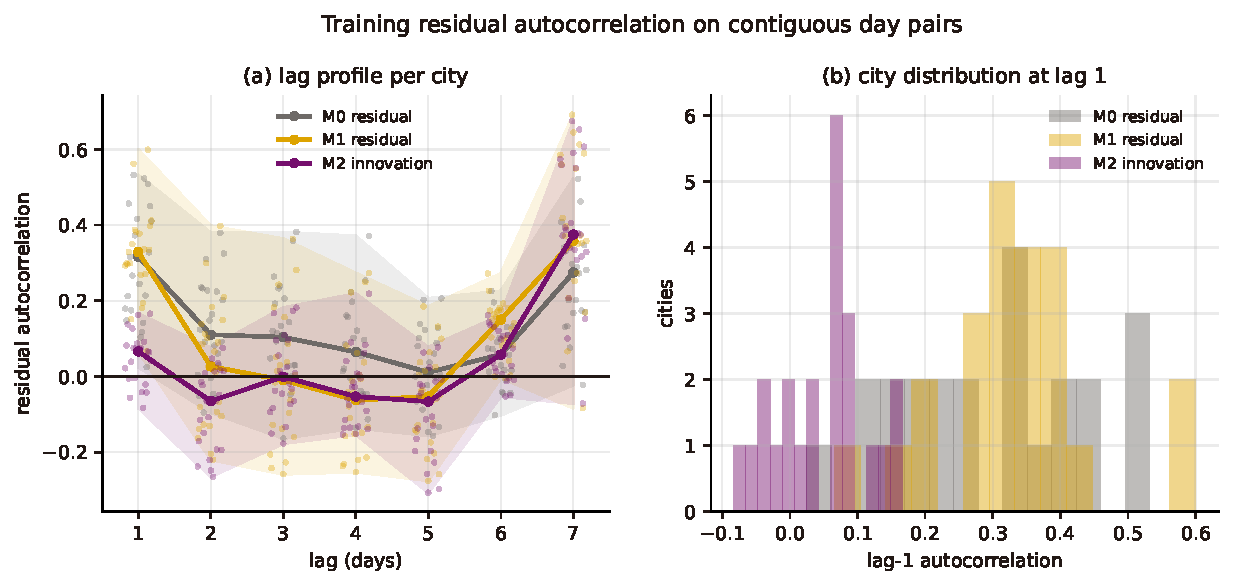
\includegraphics[width=\textwidth]{fig04_residual_acf.pdf}
\caption{Training residual autocorrelation on contiguous day pairs, first development fold. Panel (a)
lag profile per city with the median line; panel (b) the city distribution at lag one. M0 and M1 show
fitted residuals; M2 shows innovation residuals $e_{it}-\phi_ie_{i,t-1}$.}
\label{fig:acf}
\end{figure}

\paragraph{Training predictive checks.}
Because the AR(1) model conditions each day on the previous observed residual, the training-period
90\% coverage under M2 is a conditional one-step check given past observations and not a joint
replication of a whole time series. The appendix reports the coverage values and the corresponding
figure under that label.

% ===========================================================================
\section{Weather associations}
% ===========================================================================

We report the change in the conditional median of $(1+\text{usage})$ for a $+10$ mm step from the
city's median daily precipitation, and for a $+10^\circ$C step from the city's training-period mean
UTCI. On the $\log(1+\text{usage})$ scale a step of $\Delta\mu$ multiplies $(1+\text{usage})$ by
$\exp(\Delta\mu)$, so the percentage is $100(\exp(\Delta\mu)-1)$; it is computed for each posterior
draw and each city and then averaged with equal city weights. The quantity is a relative change in
the modelled location of $1+\text{usage}$, and the expected change in raw usage cannot be recovered
from a Student-$t$ log-scale model by simple back-transformation. Table~\ref{tab:effects} in the
appendix reports both full-period fits side by side.

\paragraph{Precipitation.}
Precipitation is the association this project would defend. In the 25-city full-period fit the
city-equal average is \RainMTwoMed\% (95\% interval $[\RainMTwoLo,\RainMTwoHi]$) under M2 and
\RainMZeroMed\% ($[\RainMZeroLo,\RainMZeroHi]$) under M0, and the posterior probability that the
population coefficient is negative is 1.000 in both fits. Replacing the fixed $+10$ mm step with an
observation-supported contrast, from the city median to the 90th percentile of daily precipitation,
gives \RainSupportMTwoMed\% ($[\RainSupportMTwoLo,\RainSupportMTwoHi]$) under M2 and
\RainSupportMZeroMed\% ($[\RainSupportMZeroLo,\RainSupportMZeroHi]$) under M0, so neither the sign
nor the order of magnitude depends on the contrast definition.

The association is negative in every one of the 25 cities, with city medians spanning
\RainMTwoCityMin\% to \RainMTwoCityMax\% under M2 and \RainMZeroCityMin\% to \RainMZeroCityMax\%
under M0, and the smallest city-level posterior probability of a negative coefficient is
\RainMTwoMinPNeg{} under M2 and \RainMZeroMinPNeg{} under M0. Figure~\ref{fig:rain} shows the city
estimates, each taken from its own saved fit. The spread across cities is substantial, but the city
intervals overlap and we have not tested the medians against one another, so we do not read the
ordering as evidence that two particular cities differ.

\begin{figure}[t]
\centering
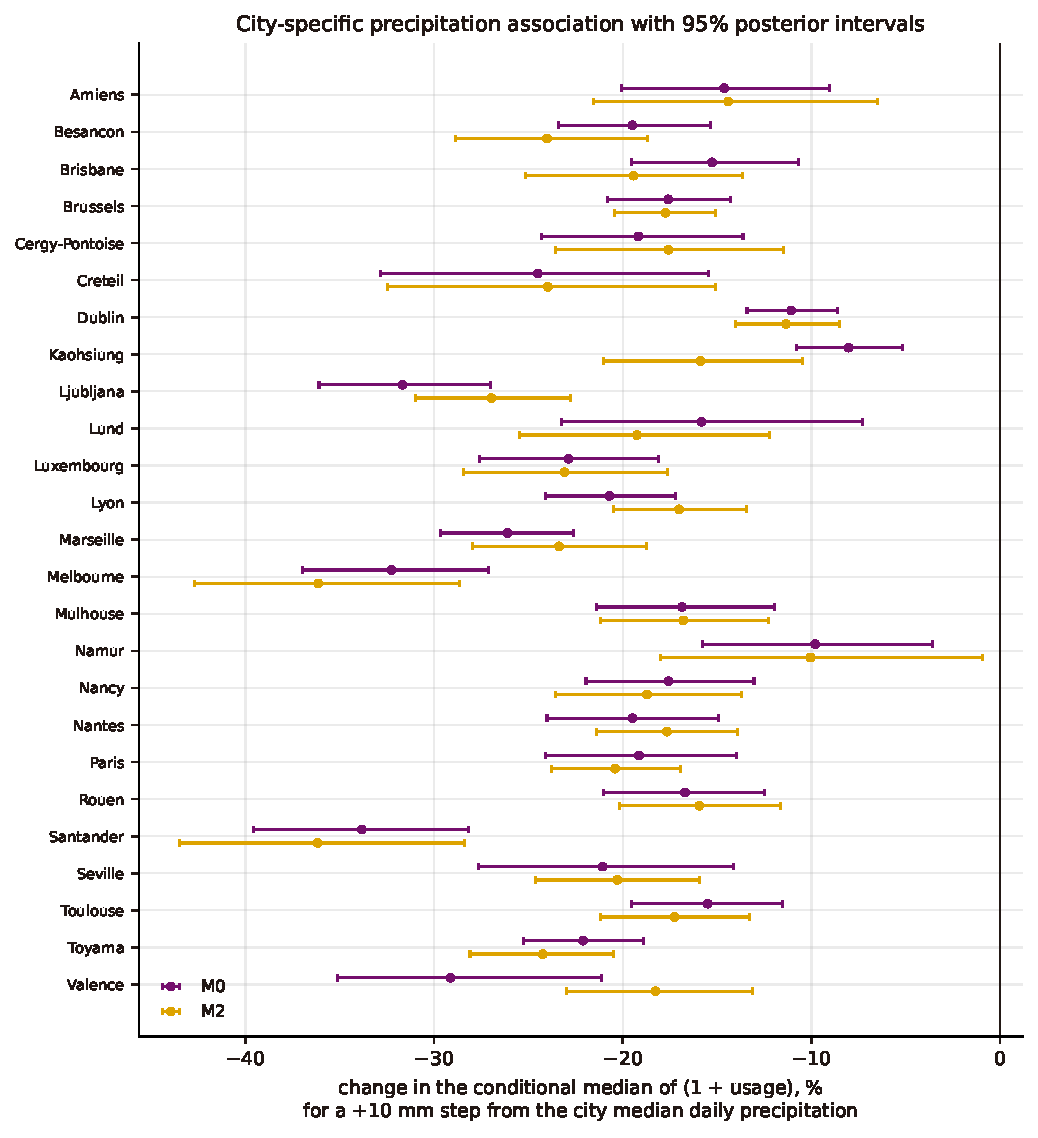
\includegraphics[width=0.78\textwidth]{fig02_rain_forest.pdf}
\caption{City-specific precipitation association in the 25-city full-period fits, shown separately
for M0 and M2. Points are posterior medians and bars are 95\% posterior intervals for the percentage
change in the conditional median of $(1+\text{usage})$ for a $+10$ mm step from the city median.}
\label{fig:rain}
\end{figure}

\paragraph{Temperature.}
Over the full period the city-equal $+10^\circ$C effect is positive under both specifications:
\TempMZeroMed\% ($[\TempMZeroLo,\TempMZeroHi]$) under M0 and \TempMTwoMed\%
($[\TempMTwoLo,\TempMTwoHi]$) under M2, on the same 25 cities and the same window. We therefore
describe the full-period comparison as a positive association rather than a reversal, and we report
the location of the response peak as uncertain rather than identified.

That uncertainty is visible in how often a concave curve peaks inside the observed support:
\PeakCitiesMZero{} of \CityCount{} cities under M0 and \PeakCitiesMTwo{} of \CityCount{} under M2
have a posterior probability above 0.95 of an interior maximum. The two counts come from different
fits and must not be combined, and the peak location is always conditional on an interior peak
existing, so we report the existence probability next to it. In both fits exactly
\ExtrapCitiesMTwo{} city has a $+10^\circ$C contrast that leaves its observed range, namely Kaohsiung,
whose study period is the warmest in the panel. Figure~\ref{fig:temperature} in the appendix shows
the curve for three cities with their observed support, and Figure~\ref{fig:allcurves} repeats all
\CityCount{} curves inside the observed range. One possible source of the variation across
specifications is that every model already carries an annual harmonic pair fitted to the same city
means, so the temperature coefficient is estimated alongside a seasonal control that shares much of
its variation; we did not run a decomposition that would confirm that overlap as the cause.

% ===========================================================================
\section{Prediction and evaluation}
\label{sec:prediction}
% ===========================================================================

\paragraph{Interval forecasts.}
Table~\ref{tab:models} is the primary prediction result. On the two development folds M2 has the
lowest block WIS, \MTwoDevOneWis{} and \MTwoDevTwoWis{} against \MZeroDevOneWis{} and
\MZeroDevTwoWis{} for M0 and \MOneDevOneWis{} and \MOneDevTwoWis{} for M1, and its mean development
WIS is \SelDevMeanWis{} against \MOneDevMeanWis{} for M1 and \MZeroDevMeanWis{} for M0. The
pre-specified selection rule, applied to the development folds only, therefore selects M2, and the
same specification is evaluated on the final window. The paired seven-day block comparison of M2
against M0 gives $[\PairDevOneLo,\PairDevOneHi]$ on the first development fold and
$[\PairDevTwoLo,\PairDevTwoHi]$ on the second; the first interval contains zero, so only the second
window shows a difference separated from zero.

\begin{table}[t]
\centering
\footnotesize
\caption{Interval forecasts for the fitted models. WIS is city-equal on the $\log(1+\text{usage})$
scale and lower is better; coverage is the city-equal 90\% interval coverage. Block and one-step
condition on different information and are not comparable.}
\label{tab:models}
% 交付用文档输入，由人工依据已保存的正式结果整理。
% 来源：runs/formal/<model>/<fold>/metrics_overall.json，字段
% tasks.block.city_equal_wis_log、tasks.block.city_equal_coverage_90、
% tasks.one_step.city_equal_wis_log、tasks.one_step.city_equal_coverage_90。
% 整理日期 2026-10-01。WIS 在 log(1 + usage) 尺度上计算，越低越好。
\begin{tabular}{lrrrrrr}
\toprule
& \multicolumn{3}{c}{City-equal WIS} & \multicolumn{3}{c}{90\% coverage (\%)} \\
\cmidrule(lr){2-4}\cmidrule(lr){5-7}
Model and task & dev 1 & dev 2 & final & dev 1 & dev 2 & final \\
\midrule
M0, block & 0.1338 & 0.2046 & 0.1957 & 76.6 & 53.8 & 75.5 \\
M1, block & 0.1320 & 0.1893 & 0.3690 & 85.1 & 70.8 & 54.9 \\
M2, block & 0.1265 & 0.1577 & 0.3394 & 88.5 & 80.1 & 60.5 \\
M2, one-step & 0.1084 & 0.1238 & 0.2085 & 90.3 & 87.2 & 72.0 \\
\bottomrule
\end{tabular}

\end{table}

\paragraph{The final window.}
The development-window advantage does not carry over. On the final block M2 scores \MTwoFinalWis{}
against \MZeroFinalWis{} for M0, and its 90\% coverage is \MTwoFinalBlockCov\% against
\MZeroFinalBlockCov\%. The one-step task shows the same pattern with \MTwoFinalStepWis{} against
\MZeroFinalStepWis{} for M0 and coverage of \MTwoFinalStepCov\% against \MZeroFinalStepCov\%. M2 has
wider mean intervals than M0, at \MTwoFinalBlockWidth{} log units against \MZeroFinalBlockWidth, but
lower coverage. These summaries indicate a mismatch between the predictive distributions and the
observations. Location error is a possible contributor, but the mechanism has not been established.
We describe this as a limitation of the specification on this window rather than as evidence about
the wider population of bike-share systems, because a single final window is one piece of evidence.
The gap is not attributed to any single term: we did not fit an M2 variant without the city trend, so
the attribution remains unverified, and the appendix records the fitted trend values and their time
scale as an observation. The mean log predictive density also carries visible Monte Carlo noise, so
we treat the WIS comparison as the more reliable summary; the appendix gives the re-run values.

\paragraph{Point forecasts against the baselines.}
The baselines are compared on log-scale MAE only. On the final block the log-scale MAE is
\MZeroFinalMaeBlock{} for M0, \BaseNaiveFinalMaeBlock{} for the seasonal naive and
\MTwoFinalMaeBlock{} for M2. On the one-step task it is \BaseArOlsFinalMaeStep{} for the city AR-OLS,
\MZeroFinalMaeStep{} for M0 and \MTwoFinalMaeStep{} for M2. All values are city-equal on the
$\log(1+\text{usage})$ scale and lower MAE is better; the complete table, including the city OLS, the
city constant and the remaining one-step values, is Table~\ref{tab:baselines} in the appendix.

% ===========================================================================
\section{Discussion and limitations}
% ===========================================================================

The precipitation association answers the first question. It is negative in every city, it is stable
across the two full-period specifications, across the fixed-step and observation-supported contrasts,
and across the three model specifications on the development fold, and it is bounded away from zero
in the city-equal summary. The city estimates differ in size, and the intervals overlap, so the
hierarchy describes a shared signal with city-level variation rather than a confirmed ranking.

The temperature result answers the second question in the negative. The full-period association is
positive under both specifications, and the peak location is not identified well enough to name a
single optimal temperature, because the estimate moves with the specification and with the contrast
definition. Both statements are conditional associations from observational data.

The time-structure result answers the third question in two parts. M2 shows lower lag-one correlation
in its innovation residuals and lower prediction scores in the development windows, but the
comparison does not establish the contribution of AR(1) alone, because the specifications differ in
several structural components. That development-window advantage does not survive into the final
window, where the block forecast is worse than the archived specification and coverage falls to
\MTwoFinalBlockCov\%. We did not retune after seeing the final window, and we do not present the
richer specification as a general improvement. Sampling reliability, residual diagnostics and
predictive performance are three separate claims, and only the first is settled by the convergence
results in Section~\ref{sec:diagnostics}.

The limitations are short and bound what the evidence supports. The study is observational and
cannot identify causal effects or climate adaptation. Each city has about one year of data, so the
study-period mean is an observation-period background rather than a long-run climate normal, and the
prediction roster is conditioned on full-period activity, so the evaluation describes continuously
operating systems. Usage is inferred from inventory changes and may include rebalancing moves. Both
prediction tasks condition on realised weather and therefore say nothing about a forecast that has to
predict the weather first, and the final block was inspected before this analysis, which we note
wherever its numbers appear. The Student-$t$ log-scale likelihood permits negative log usage and the
expected usage does not exist after the exponential transform, so we report medians and predictive
quantiles only. Finally, the three models differ in several structural respects at once, so the
comparison identifies the value of the package rather than the value of any single term.

% ===========================================================================
\section*{Contribution statement}
% ===========================================================================

XUE Yantong searched for data, selected the topic, designed the experiments, developed code,
ran the experiments, conducted the main statistical analysis, and prepared the report and presentation.
WANG Ziyu and ZHAO Jiashen contributed to data processing, code development and
checking, and verification of the report and slides.

\bibliographystyle{plainnat}
\bibliography{references}

\newpage
\appendix
\section{Appendix}

\paragraph{Panel by city.}
Figure~\ref{fig:overview} shows the three rosters, the system sizes and the observation windows.
Every city except Kaohsiung and Melbourne starts on 2017-01-01 or 2017-01-02 and ends on 2017-12-31,
so 21 of the 23 prediction cities contribute 365 days and Brisbane and Toyama contribute 364.
Kaohsiung has 363 recorded days and one missing date, 2016-09-27, the only gap inside a study period
anywhere in the panel; it affects only the full-period fit for the 25-city roster, because the AR
recursion restarts after any calendar gap longer than one day. Usage is recorded as a half-integer on
$4{,}936$ city-days.

\begin{figure}[h]
\centering
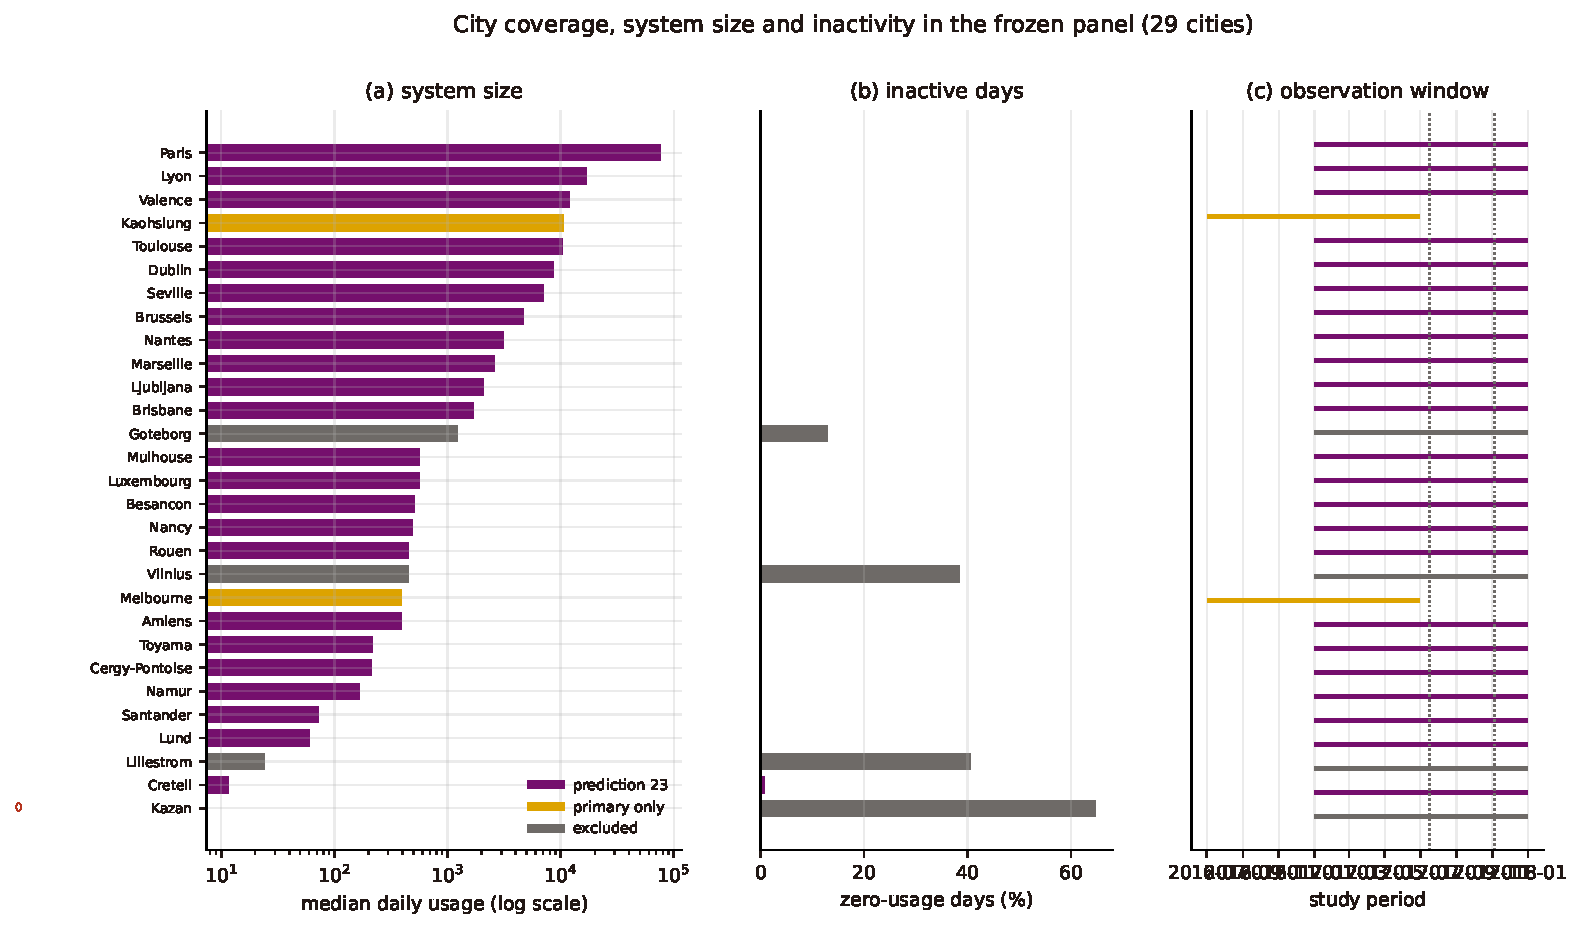
\includegraphics[width=\textwidth]{fig01_city_overview.pdf}
\caption{The frozen panel by city, ordered by median daily usage. Panel (a) system size on a log
scale, panel (b) share of zero-usage days, panel (c) observation window with the development and
final cutoffs marked. Colours separate the 23 prediction cities, the two primary-only cities and the
four excluded systems.}
\label{fig:overview}
\end{figure}

\paragraph{Metric definitions.}
The WIS uses the fixed 50/80/90/95\% central intervals, following \citet{bracher2021evaluating} and
the scoring-rule background in \citet{gneiting2007strictly}. The mean log predictive density is the
average log density at the realised value, the log-scale MAE is the average absolute error in
$\log(1+\text{usage})$, and the 90\% interval coverage is the share of realised values inside the
central 90\% interval. The normalised error divides each city's log-scale absolute error by that
city's training-period seven-day seasonal naive error. The four baselines are a city constant, a
seven-day seasonal naive forecast, a city OLS with parameter uncertainty, and a city AR-OLS.

\paragraph{Implementation details of the fitted models.}
The stored configuration carries a \texttt{beta\_trend\_city\_sd} entry of $0.2$. The constructor
does not read it: it passes \texttt{beta\_trend\_population\_sd} $=0.3$ to the varying-coefficient
helper, which uses that single value for both the population mean and the between-city scale, so the
fitted trend prior is $\mathcal{N}(0,0.3)$ with a $\text{HalfNormal}(0.3)$ group scale. We report the
fitted value and leave the configuration file unchanged so that the saved run records stay as they
were produced. The first observation of every contiguous date segment uses a Student-$t$
distribution with scale $\sigma_i\sqrt{\nu/((\nu-2)(1-\phi_i^2))}$, which is wider than the
stationary innovation scale.

\paragraph{Prior predictive check.}
The saved prior predictive draw for M2 on the first development fold gives an intercept-only
negative-usage fraction of \PriorNegIntercept\%, which describes the city intercepts alone. The
supplementary full check stored at \texttt{logs/review-20261001/followup\_checks.json}, with its
implementation at \texttt{logs/review-20261001/audit\_followup.py}, uses 1{,}000 parameter draws and
places \PriorNegJoint\% of the log response below zero, with log-response quantiles
$[\PriorLogLow,\ \PriorLogHigh]$ against an observed range of $0$ to $\ObsLogHigh$. The corresponding
full check was not run for M0.

\paragraph{Reparameterisations.}
Three components were reparameterised for computational reasons without changing the target
distribution. The city intercept hierarchy and the city noise scale are written in centred form, and
the shared weekday effect uses an orthonormal sum-to-zero basis with six free contrasts in place of a
centred seven-vector that carried a direction the likelihood does not identify. Each change is a
reparameterisation of the same prior and likelihood, and each was adopted after the original form
failed the acceptance rule above.

\paragraph{Fitted time-structure parameters.}
In the M2 full-period fit the persistence parameter has a median of \PhiMTwoMed{} with a 95\%
interval of $[\PhiMTwoLo,\PhiMTwoHi]$ across cities and posterior draws, so the residual state carries
information for roughly one to two days. The degrees of freedom are \NuMTwoMed{}
$[\NuMTwoLo,\NuMTwoHi]$, which keeps the innovation distribution heavy-tailed and places the fitted
model away from the Gaussian limit. Under M0 the training-period 90\% predictive coverage is
\MZeroDevOneTrainCov\% and under M2 it is \MTwoDevOneTrainCov\%; Figure~\ref{fig:ppc} shows the M2
check by city.

\paragraph{Full-period association table.}
Table~\ref{tab:effects} reports both full-period fits side by side, including the
observation-supported contrast and the count of cities with an interior temperature peak.

\begin{table}[h]
\centering
\footnotesize
\caption{Weather associations in the 25-city full-period fits. Entries are city-equal averages of the
percentage change in the conditional median of $(1+\text{usage})$, with 95\% posterior intervals. M0
and M2 are separate fitted specifications, reported from their own saved results.}
\label{tab:effects}
% 交付用文档输入，由人工依据已保存的正式结果整理，不通过 src/make_report_inputs.py 写出。
% 来源：runs/formal_20260930/M0/full/effects.json 与 runs/formal_20260930/M2/full/effects.json。
% 字段：rain_10mm_city_equal_percent、rain_support_city_equal_percent、
% temp_10c_city_equal_percent、temp_support_city_equal_percent、
% cities_with_interior_maximum_probability_above_0_95、cities_with_temp_10c_outside_support。
% 整理日期 2026-10-01。区间为 95% 后验可信区间。
\begin{tabular}{lrr}
\toprule
Contrast & M0 & M2 \\
\midrule
Precipitation: city median $+10$ mm & $-19.98$ & $-20.21$ \\
 & $[-21.07,\,-18.89]$ & $[-21.37,\,-18.99]$ \\
Precipitation: median to 90th percentile & $-16.40$ & $-16.99$ \\
 & $[-17.28,\,-15.53]$ & $[-18.02,\,-15.95]$ \\
UTCI: city mean $+10^\circ$C & $5.22$ & $6.16$ \\
 & $[3.67,\,6.76]$ & $[4.12,\,8.32]$ \\
UTCI: 25th to 75th percentile & $19.89$ & $14.04$ \\
 & $[17.44,\,22.47]$ & $[11.11,\,17.27]$ \\
Cities with interior peak, $P>0.95$ & 15 of 25 & 5 of 25 \\
Cities leaving the observed range at $+10^\circ$C & 1 of 25 & 1 of 25 \\
\bottomrule
\end{tabular}

\end{table}

\paragraph{Development-fold temperature comparison.}
On the first development fold, which is a 23-city training window with a \BlockDays-day test block,
the same $+10^\circ$C quantity is \TempMZeroDevOneMed\% ($[\TempMZeroDevOneLo,\TempMZeroDevOneHi]$)
under M0, \TempMOneDevOneMed\% ($[\TempMOneDevOneLo,\TempMOneDevOneHi]$) under M1 and
\TempMTwoDevOneMed\% ($[\TempMTwoDevOneLo,\TempMTwoDevOneHi]$) under M2, while the precipitation
association is almost unchanged across the same three fits at \RainMZeroDevOneMed\%,
\RainMOneDevOneMed\% and \RainMTwoDevOneMed\%. The observation-supported temperature contrast over
the full period gives \TempSupportMZeroMed\% ($[\TempSupportMZeroLo,\TempSupportMZeroHi]$) under M0
against \TempSupportMTwoMed\% ($[\TempSupportMTwoLo,\TempSupportMTwoHi]$) under M2, and across the
panel the observed daily mean UTCI runs from \ObsUtciMinC{} to \ObsUtciMaxC{} degrees. The three
development-fold values come from a different window and a different roster from the full-period
values, and the two groups are not comparable with each other.

\begin{figure}[h]
\centering
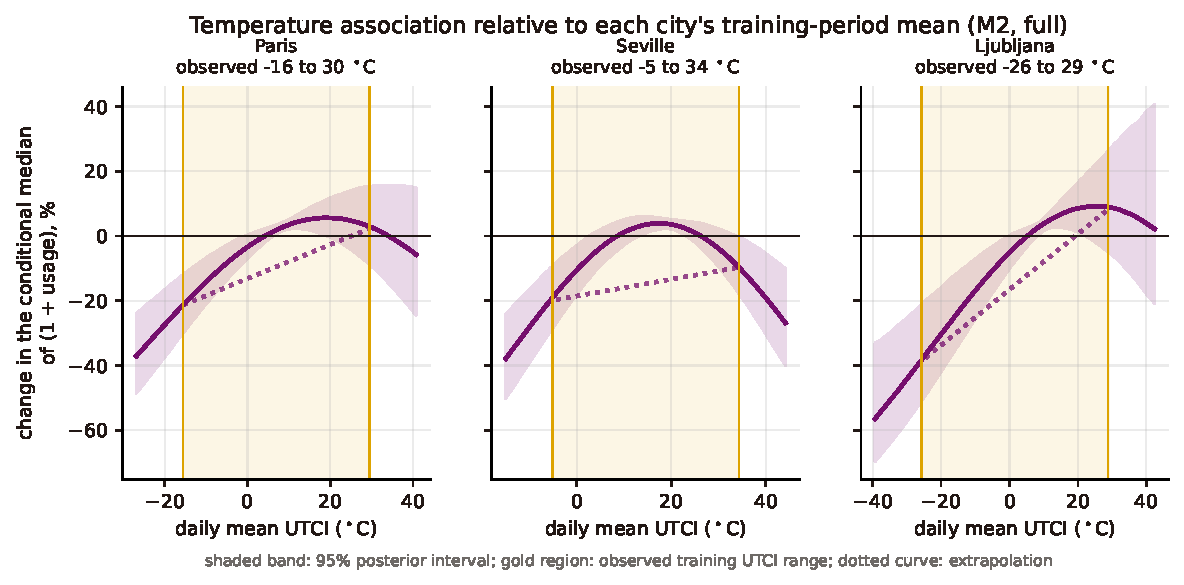
\includegraphics[width=\textwidth]{fig03_temperature_curves.pdf}
\caption{Temperature association relative to each city's training-period mean in the 25-city
full-period M2 fit. Shaded bands are 95\% posterior intervals; the gold region is the observed
training UTCI range; dotted segments are extrapolation beyond that range.}
\label{fig:temperature}
\end{figure}

\begin{figure}[h]
\centering
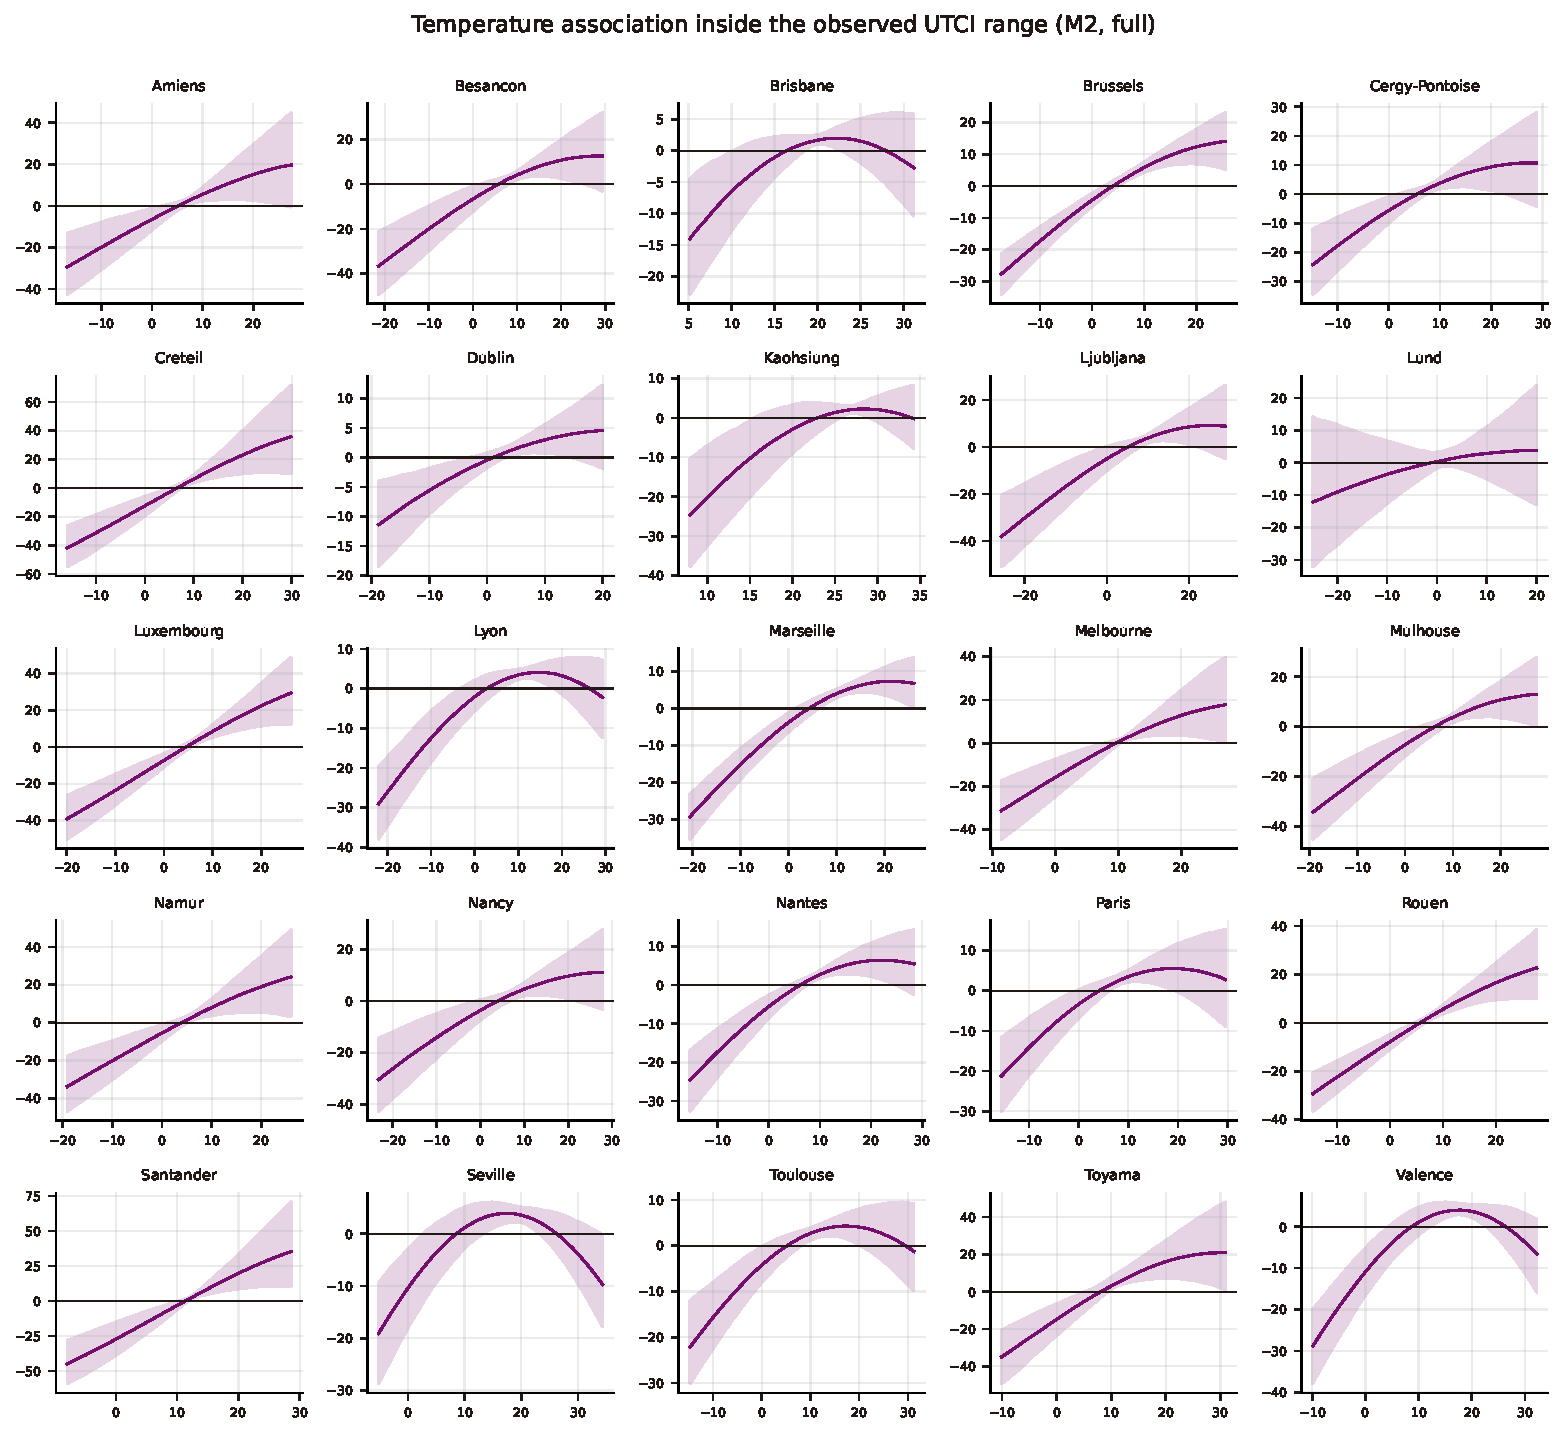
\includegraphics[width=\textwidth]{figA2_all_city_curves.pdf}
\caption{Temperature association inside the observed UTCI range for all 25 cities in the M2
full-period fit.}
\label{fig:allcurves}
\end{figure}

\paragraph{Point-forecast table.}
Table~\ref{tab:baselines} reports the full final-window comparison, including the city OLS and the
city constant, and Table~\ref{tab:baselines_dev} reports the same comparison on the two development
folds.

\begin{table}[h]
\centering
\footnotesize
\caption{Point-forecast error on the final window, in log-scale MAE on $\log(1+\text{usage})$,
city-equal and lower is better. M0 and M2 come from the independent recomputation of their saved
daily predictions; the four baselines come from a supplementary check completed before this
write-up.}
\label{tab:baselines}
% 交付用文档输入，由人工依据已保存的正式结果整理。
% 来源：logs/review-20261001/recomputed_metrics.csv 中 M0 与 M2 的 city_equal_mae_log，
% 以及 logs/review-20261001/followup_checks.json 中 final_baselines_existing_implementation
% 的 mae_log。整理日期 2026-10-01。
% 全部数值在 log(1 + usage) 尺度上计算，城市等权汇总，越低越好。
% 行序按 block MAE 从小到大排列。
\begin{tabular}{lrr}
\toprule
Method & Block MAE & One-step MAE \\
\midrule
M0 & 0.3207 & 0.3207 \\
Seasonal naive, 7-day lag & 0.4252 & 0.3421 \\
City AR-OLS & 0.5192 & 0.3197 \\
City OLS, parameter uncertainty & 0.5208 & 0.5208 \\
M2 & 0.5547 & 0.3601 \\
City constant & 0.5551 & 0.5551 \\
\bottomrule
\end{tabular}

\end{table}

\begin{table}[h]
\centering
\footnotesize
\caption{Point-forecast error in log-scale MAE on $\log(1+\text{usage})$, city-equal, lower is
better, recomputed from the saved daily predictions.}
\label{tab:baselines_dev}
% 交付用文档输入，由人工依据已保存的正式结果整理，不通过 src/make_report_inputs.py 写出。
% 来源：logs/review-20261001/recomputed_metrics.csv 中 dev1 与 dev2 的 city_equal_mae_log，
% 该表由独立核验脚本从已保存的逐日预测复算。整理日期 2026-10-01。
% 全部数值在 log(1 + usage) 尺度上计算，城市等权汇总，越低越好。
% 基线在多步任务上的区间未累计未来创新，因此本表只用于点预测比较。
\begin{tabular}{llrr}
\toprule
Fold & Method & Block MAE & One-step MAE \\
\midrule
dev 1 & City constant & 0.3757 & 0.3757 \\
dev 1 & Seasonal naive, 7-day lag & 0.2602 & 0.2298 \\
dev 1 & City OLS, parameter uncertainty & 0.3314 & 0.3314 \\
dev 1 & City AR-OLS & 0.3309 & 0.2553 \\
dev 1 & M0 & 0.2571 & 0.2571 \\
dev 1 & M2 & 0.2503 & 0.2104 \\
dev 2 & City constant & 0.3665 & 0.3665 \\
dev 2 & Seasonal naive, 7-day lag & 0.2664 & 0.2405 \\
dev 2 & City OLS, parameter uncertainty & 0.3131 & 0.3131 \\
dev 2 & City AR-OLS & 0.3110 & 0.2278 \\
dev 2 & M0 & 0.3701 & 0.3701 \\
dev 2 & M2 & 0.3239 & 0.2540 \\
\bottomrule
\end{tabular}

\end{table}

\paragraph{Predictive integration stability.}
Re-running the same predictive integration for M2 with 800 posterior draws instead of 400 and a
different seed gives a development-fold WIS of \IntegDevOneWisNew{} against the saved
\IntegDevOneWisSaved{} and a final-fold WIS of \IntegFinalWisNew{} against the saved
\IntegFinalWisSaved{}, with a maximum absolute per-day density change of \DensityStabilityDevOne{} and
\DensityStabilityFinal. The recomputed WIS values are close to the saved values, and the main
model-comparison conclusion is unchanged; the results are not identical at the listed decimal places,
and the per-day densities carry the larger Monte Carlo variation.

\paragraph{Fitted city trend.}
The city trend coefficients of the M2 final-window fit are positive in all \PredCityCount{} prediction
cities, with city medians from \TrendCityMin{} to \TrendCityMax{} per 100 days and a city median of
\TrendCityMedian. The final test window lies \TrendWindowLow{} to \TrendWindowHigh{} trend units
beyond the training centre, so for a median city the trend term adds roughly \TrendLogLow{} to
\TrendLogHigh{} log units across the whole window. This is consistent with the trend contributing to a
location error in the final window, but we did not fit an M2 variant without the trend, so the
mechanism is not established.

\paragraph{Additional figures.}
Figure~\ref{fig:scores} shows the scores behind Table~\ref{tab:models} across folds and tasks.
Figure~\ref{fig:trajectories} shows the final-window block forecasts for three cities chosen before
the plot was drawn: Paris, Lund, and the city with the median WIS. Figure~\ref{fig:convergence} gives
the convergence diagnostics across all parameters, Figure~\ref{fig:sensitivity} the weather
prior-scale check on the first development fold, and Figure~\ref{fig:ppc} the training conditional
predictive check.

\begin{figure}[h]
\centering
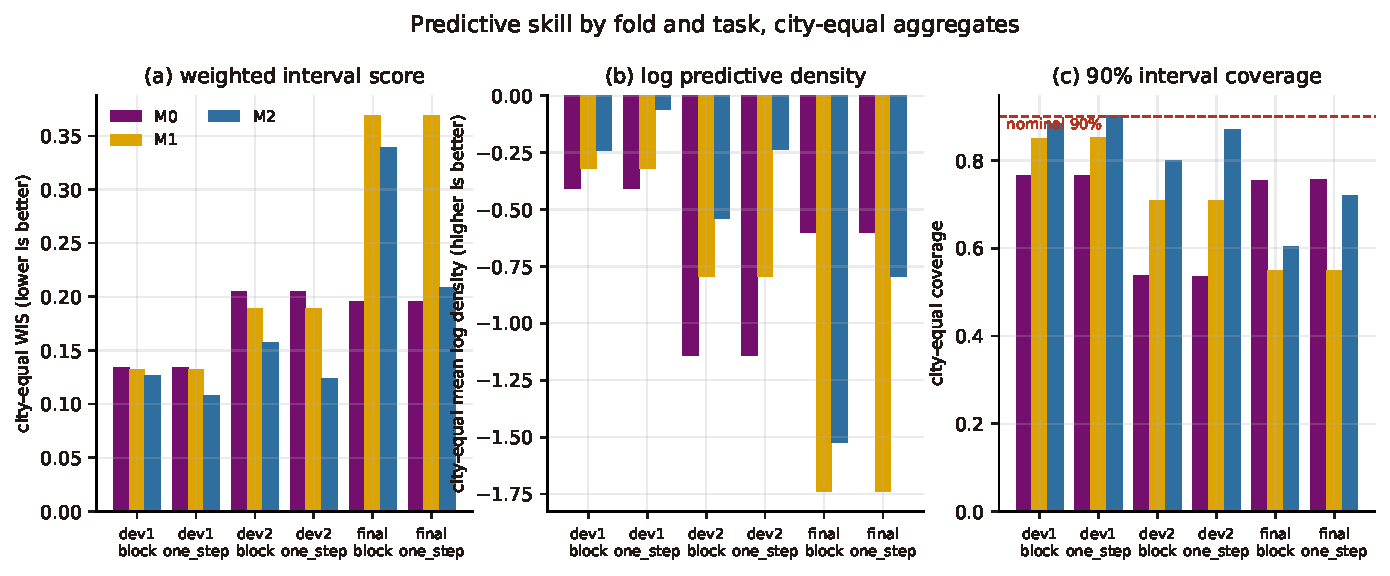
\includegraphics[width=\textwidth]{fig05_forecast_scores.pdf}
\caption{Predictive skill by fold and task. Panel (a) city-equal WIS, panel (b) city-equal mean log
predictive density, panel (c) city-equal 90\% coverage with the nominal level marked.}
\label{fig:scores}
\end{figure}

\begin{figure}[h]
\centering
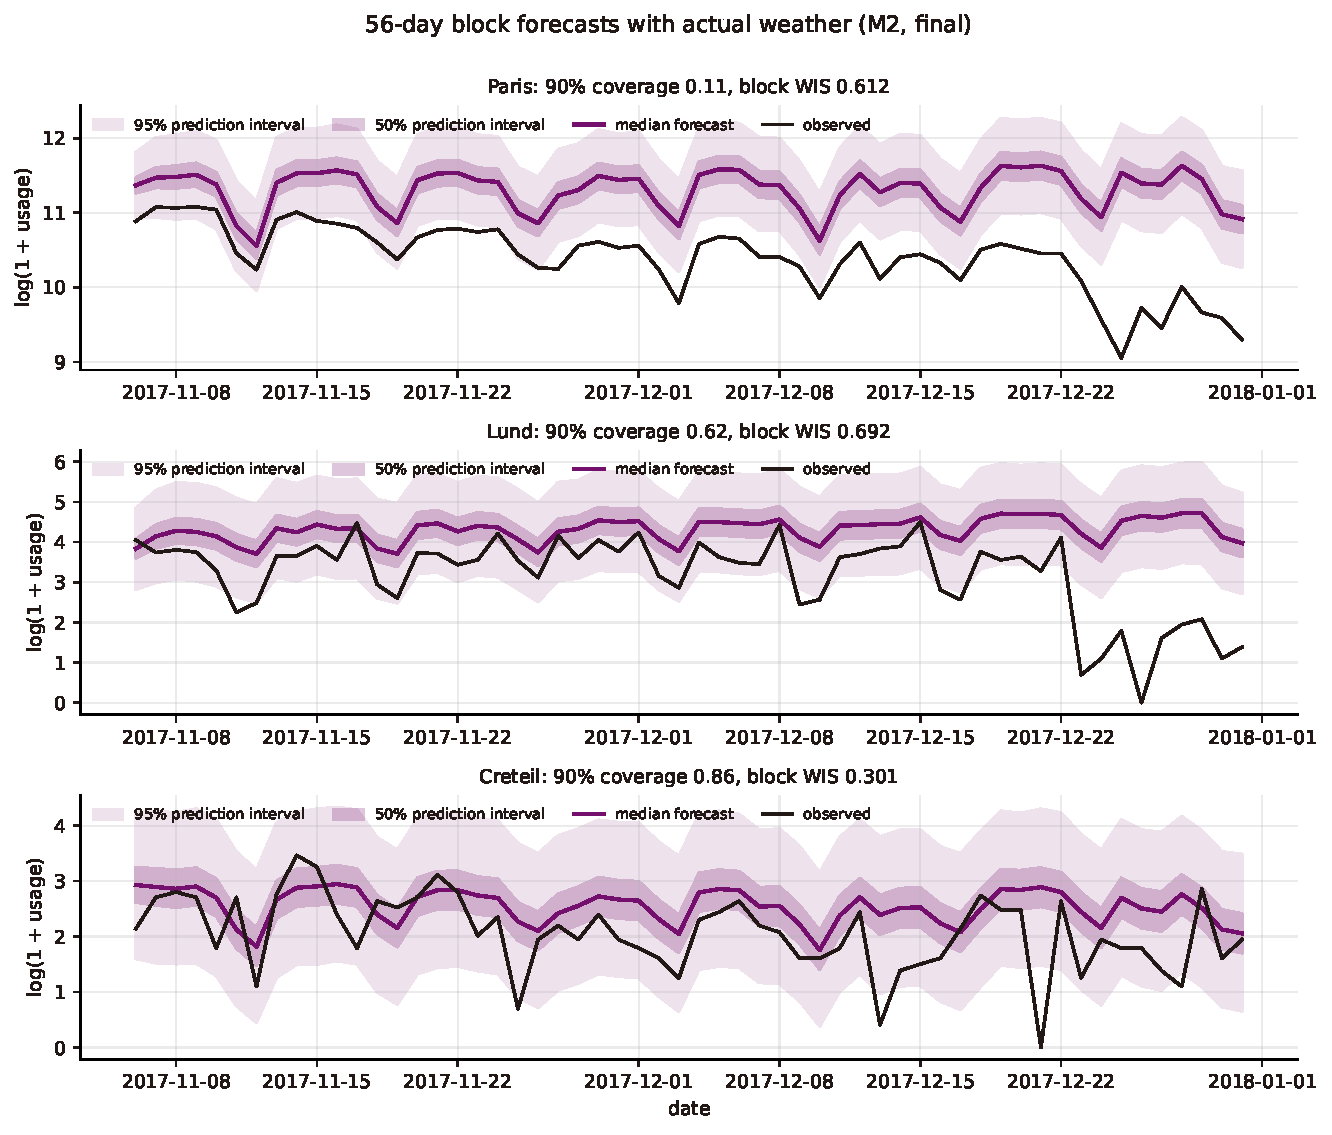
\includegraphics[width=\textwidth]{fig06_city_trajectories.pdf}
\caption{56-day block forecasts with realised weather on the final window for Paris, Lund and the
median-WIS city, under M2. Bands are 50\% and 95\% prediction intervals; the black line is the
observed series.}
\label{fig:trajectories}
\end{figure}

\begin{figure}[h]
\centering
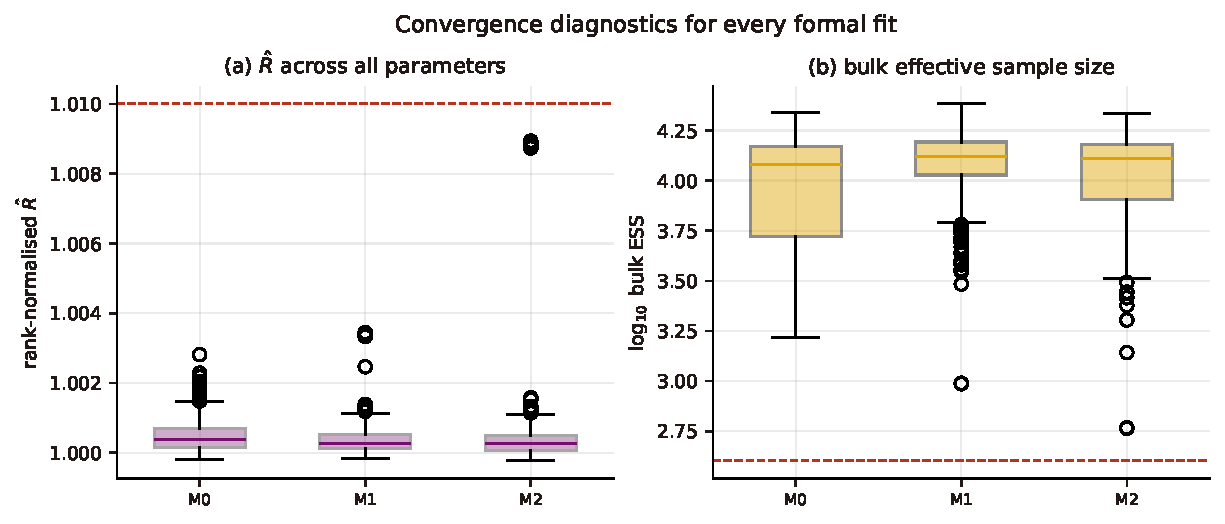
\includegraphics[width=\textwidth]{figA3_convergence.pdf}
\caption{Convergence diagnostics for the M0, M1 and M2 fits on the first development fold, across all
parameters.}
\label{fig:convergence}
\end{figure}

\begin{figure}[h]
\centering
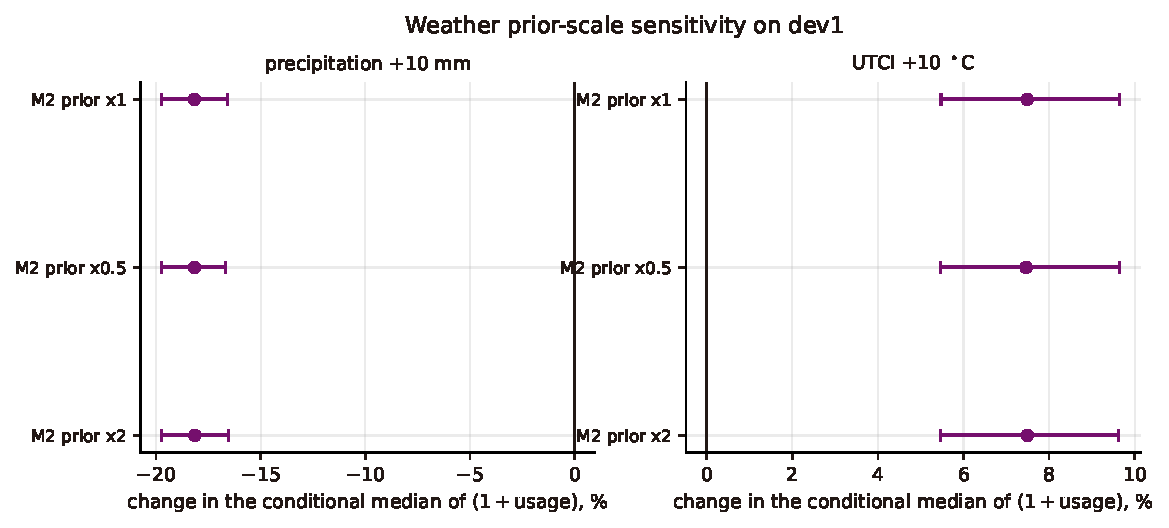
\includegraphics[width=\textwidth]{figA4_sensitivity.pdf}
\caption{Weather prior-scale sensitivity for M2 on the first development fold. The rain association is
\SensRainBase\% at the baseline scale, \SensRainHalf\% at half scale and \SensRainDouble\% at double
scale; the temperature association is \SensTempBase\%, \SensTempHalf\% and \SensTempDouble\%.}
\label{fig:sensitivity}
\end{figure}

\begin{figure}[h]
\centering
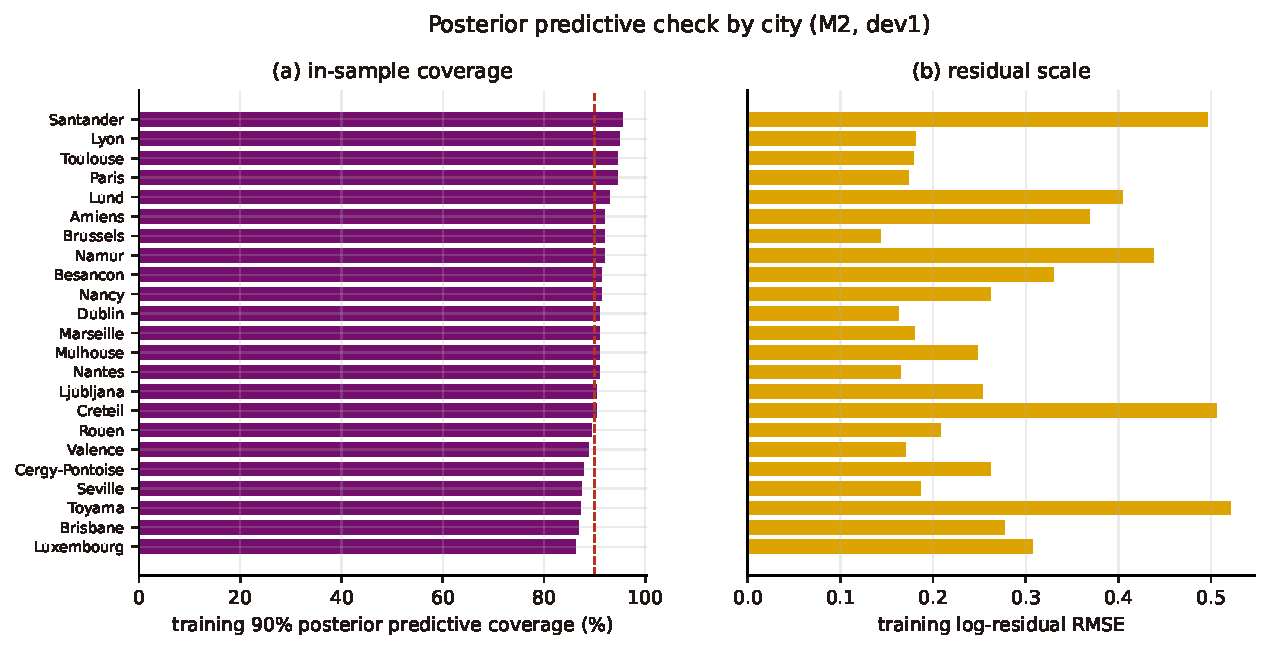
\includegraphics[width=\textwidth]{figA5_posterior_predictive.pdf}
\caption{Training conditional predictive check by city for M2 on the first development fold. Each day
is conditioned on the previous observed residual, so this is not a joint replication of a whole time
series.}
\label{fig:ppc}
\end{figure}

\paragraph{Software and reproduction.}
Models were fitted with PyMC 6.3.2 \citep{abrilpla2023pymc} and nutpie 0.16.11 \citep{nutpie} on
PyTensor 3.3.2. Posterior summaries, rank-normalised $\hat{R}$ and effective sample sizes use ArviZ
\citep{kumar2019arviz}. Numerics use NumPy \citep{harris2020numpy}, pandas \citep{mckinney2010pandas}
and SciPy. Figures use Matplotlib \citep{hunter2007matplotlib}. The exact versions of every run are
recorded in its \texttt{config.json}. The working directory contains the configuration, the source,
the tests, the run outputs, the tables and the figures, together with a cleaned copy of the daily
panel at \texttt{data/bikeshare\_weather\_daily.csv}, byte-identical to the frozen input used for
every saved run and checked by SHA-256 before each fit. The pipeline is driven by \texttt{src/run.py}
subcommands and described in \texttt{README.md}; the test suite asserts that the splits respect the
cutoffs, that training standardisation does not depend on test rows, that block forecasts cannot read
realised test usage, and that the AR recursion reduces to independent innovations when $\phi=0$.

\end{document}
